\title{Final Project Report}
\author{
  Mukesh Jha\\
  \texttt{mjha@masdar.ac.ae}
  	\and
  Bikash Joshi\\
  \texttt{bjoshi@masdar.ac.ae}
  	\and
  Puskar Budhathoki\\
  \texttt{pbudhathoki@masdar.ac.ae}
  	\and
  Abraham Xiao\\
  \texttt{yxiao@masdar.ac.ae}  
  }

\date{\today}

\documentclass[12pt]{article}

\usepackage[margin=0.75in]{geometry}
\usepackage{booktabs}
\usepackage{graphicx}
\usepackage{amsmath}
\usepackage{amsfonts}
\usepackage{hyperref}
\usepackage{float}

% Some house keeping


\begin{document}
\maketitle

\section{Introduction}
It was a successful team work which culminated in implementation of five features. All the team-members contributed with their full capacity. We worked as a closely related team and implemented the project with concept of agile software development paradigm. 

 

\section{Feature: Backup-Restore}
This feature enables user to create the backup of application data and also helps to restore the it. It allows interactive GUI for users to facilitate the functionality of this feature. 

\begin{enumerate}
\item \href{https://bitmessage.org/forum/index.php/topic,3306.0.html}{Forum Thread} 
\item \href{https://github.com/Bitmessage/PyBitmessage/pull/554}{Pull Request}
\end{enumerate}

\subsection{User Story}
\underline{\bf{Title:}} \\ Backup/Restore Data\\
\underline{\bf{Description:}}\\
A user should be able to create a backup his Inbox, Sent and other application data and conveniently restore some key and message from remote location through intuitive GUI. This feature also provides selective restoration of only Inbox. \\
\underline{\bf{Acceptance criteria:}}\\
The Backup/Restore mechanism should have the ability to backup data from user specified location.\\
The feature should be able to Backup data at "./Backup" folder by default.\\
After restoring the data, earlier message should be flushed.\\

\subsection{Changelog}
\date{\today}
 
\begin{itemize}
\item bitmessageqt.py  : Added a class NewBackupRestoreDialog and functionality of backup, restore and delete-backup.
\item backuprestore.py : Introduced this to create the GUI.
\item backuprestore.ui : Introduced this file to give other developers easy access to modify the GUI
\end{itemize}

To implement this feature, we created a GUI to enable users for preference. With active inputs from the bitmessage community, We created this feature as per their requirements.\\

\noindent\underline{\bf{The formal documentation of the class:}}\\
\large{Class Reference [NewBackupRestore module]}

The NewBackupRestore class specifies a functionality associated with GUI form created by backuprestore.py. It consists of following methods: \\
\large{\underline{Methods}}
\begin{itemize}
\item Boolean verify\textunderscore form(self): Verifies the inputs given by the user before implementing it.
\item checkPermission(self): checks the permission if the task assigned by the use is feasible or not.
\item BackupRestoreaccepted(self): implements the backup, restore and delete feature. 
\item selectDirectory(self): module to enable browser to brows through the directory structure.
\end{itemize}

\subsection{Screen-Shots}
The GUI of the implemented feature:
\begin{figure}[H]
\begin{center}
    {\label{fig:1} 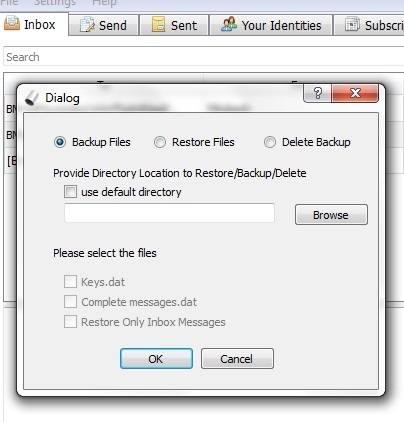
\includegraphics[width=8cm,height=6cm]{2_gui_backup_restore.jpg}}   
  \centering  \caption{GUI}
  \end{center}
\end{figure}


\begin{figure}[H]
\begin{center}
    {\label{fig:1} 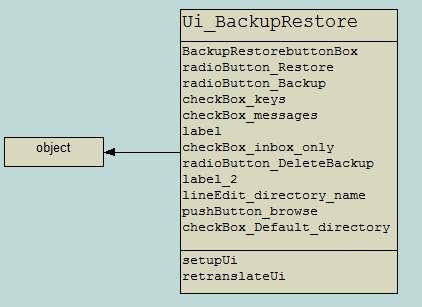
\includegraphics[width=8cm,height=6cm]{BakcupRestore.jpg}}   
  \centering  \caption{ Class Diagram } 
  \end{center}
\end{figure}

\begin{figure}[H]
\begin{center}
    {\label{fig:1} 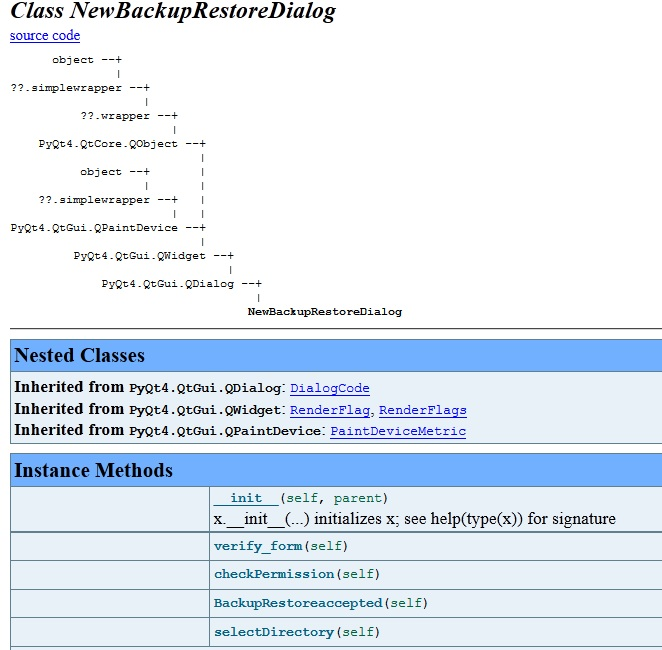
\includegraphics[width=10cm,height=8cm]{NewBackupRestoreDialogClass.jpg}}   
  \centering  \caption{Method Diagram}
  \end{center}
\end{figure}

%% Bikash

\section{Feature: add option `add Subscription to Address book’  in the context menu of subscription list}

\subsection{Introduction}
This feature allows the users to add the selected subscription (from the subscription list) to the address book. We have added “Add Subscription to Address Book” option in the context menu for Subscriptions. When a user selects a subscription from the subscription list, he can see this option in the context menu which can be viewed by right clicking the selected subscription. So, when the user clicks this option, it will first check if the selected address is already present in the Address book or not. If it is already present in the address book then it displays an error message “Error: You cannot add the same address to your address book twice. Try renaming the existing one if you want.”  But if the address is not present in the address book, it adds the selected address and corresponding label to the Address Book. And it displays a success message “Entry added to the Address Book. Edit the label to your liking”. Detailed description and screenshots for this feature are also shown in:
\begin{enumerate}
\item \href{https://bitmessage.org/forum/index.php?topic=3313.0}{Forum Thread} 
\item \href{https://github.com/Bitmessage/PyBitmessage/pull/555}{Pull Request} 

\end{enumerate}

\subsection{User-Story}
\begin{itemize}
\item Title: Add new subscriptions to address book

\item Description: As a bitmessage user, I want the functionality to add new subscripitions to address book list so that I can save the subscription list in the Address book for future use. 

\item Acceptance Criteria: The Subscription list contains the address of subscriptions. Adding the addresses from subscription list to address book, should copy the selected address from subscription list and make a new record in the Address book.
\end{itemize}

\subsection{Change Log}

\begin{itemize}
\item Class: To implement this feature we have made changes to the init.py (bitmessageqt.py) class in the bitmessageqt package. We added pop up menu option for `add Subscription to Address book' in the context menu of Subscription.
\item Method: We have added a method on\_action\_SubscriptionAddSenderToAddressBook to bitmessageqt.py class. This contains the main functionality for adding selected subscription to the address book.
\end{itemize}

\subsection{Screenshots:}

\begin{figure}[H]
\begin{center}
    {\label{fig:1} 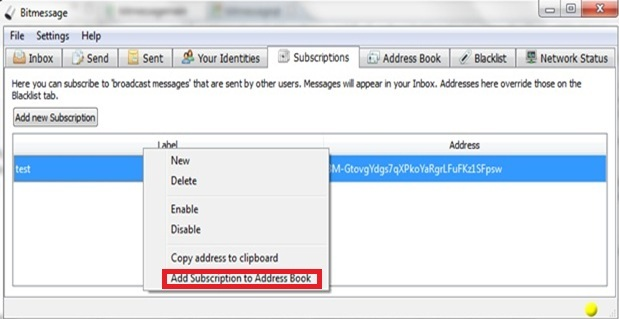
\includegraphics[width=12cm,height=5cm]{F1_1.jpg}}   
  \centering  \caption{ Screen showing “Add Subscription to Address book” option in the context menu for subscription}
  \end{center}
\end{figure}

\begin{figure}[H]
\begin{center}
    {\label{fig:1} 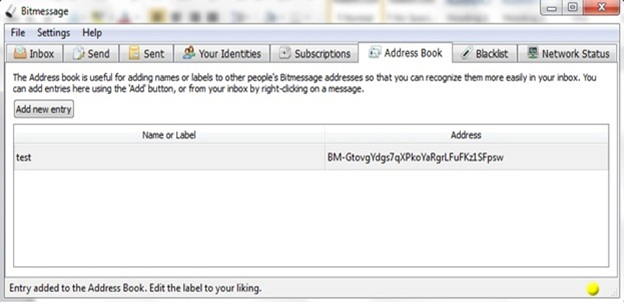
\includegraphics[width=12cm,height=5cm]{F1_2.jpg}}   
  \centering  \caption{Screen showing the selected subscription added to the address book when the selected subscription is not already present in the address book}
  \end{center}
\end{figure}

\begin{figure}[H]
\begin{center}
    {\label{fig:1} 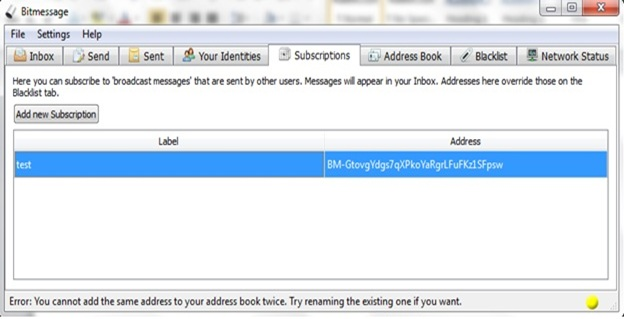
\includegraphics[width=12cm,height=5cm]{F1_3.jpg}}   
  \centering  \caption{Screen showing the error message when the selected subscription is already present in the address book}
  \end{center}
\end{figure}

\section{Feature: When replying to a message, populate the 'from' field}

\subsection{Introduction}
A user can have more than one identity. Each identity has a unique address, label and icon. Currently, when the user replies to a message the 'from' field is left blank.  So, when user replies to a message sent to one of his addresses, the 'from' field should show the corresponding user label and icon. This feature helps to populate the 'from' field with the corresponding label and icon for the address to which the message was sent. 

When the user selects a message in the 'inbox' and selects the 'reply' option by right clicking on it, the ‘from’ field populates the corresponding label for the address of the user in which the message was sent to, whereas the address is displayed in the label adjacent to the 'from' field. If that address does not have an address then it only displays the icon for that address in the 'from' field. Detailed description and screenshots for this feature are also shown in:
\begin{enumerate}
\item \href{https://bitmessage.org/forum/index.php?topic=3384.0}{Forum Thread} 
\item \href{https://github.com/Bitmessage/PyBitmessage/pull/581}{Pull Request} 

\end{enumerate}

\subsection{User-story:}
\begin{itemize}
\item Title: Populate 'from field’ while replying to a message.

\item Description: As a bitmessage software user, I need the ability to populate the 'from field’ while replying to a message so that I can easily visualize the sender and receiver addresses in the reply message.

\item Acceptance criteria: The message inbox has the ability to 'Reply' an existing message. The 'Reply' message will have a text field to populate the 'from field’

\end{itemize}

\subsection{Change Log:}
\begin{itemize}
\item Class: To implement this feature we have made changes to the init.py (bitmessageqt.py) class in the bitmessageqt package. 
\item Method: We have modified the on\_action\_InboxReply function in the bitmessageqt.py class. In this method we have added the code to set the index of ‘from’ field label and icons to corresponding address to which the message was sent.
\end{itemize}

\subsection{Screenshots:}

\begin{figure}[H]
\begin{center}
    {\label{fig:1} 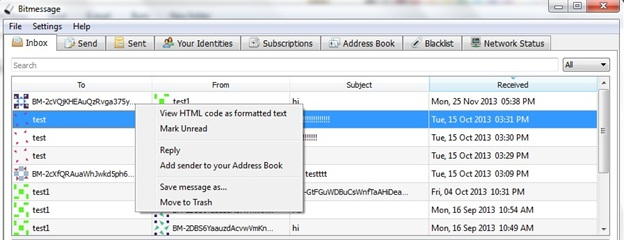
\includegraphics[width=12cm,height=5cm]{F2_1.jpg}}   
  \centering  \caption{Screen showing when user replies to a message sent to his address having label and icon}
  \end{center}
\end{figure}

\begin{figure}[H]
\begin{center}
    {\label{fig:1} 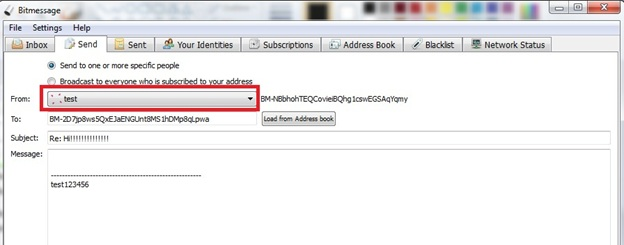
\includegraphics[width=12cm,height=5cm]{F2_2.jpg}}   
  \centering  \caption{Screen showing the 'from' field populated with corresponding label and icon}
  \end{center}
\end{figure}

\begin{figure}[H]
\begin{center}
    {\label{fig:1} 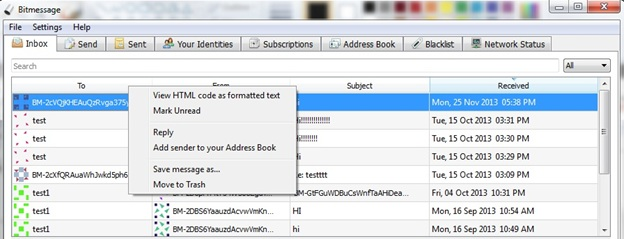
\includegraphics[width=12cm,height=5cm]{F2_3.jpg}}   
  \centering  \caption{Screen showing when user replies to message sent to his address not having a label}
  \end{center}
\end{figure}

\begin{figure}[H]
\begin{center}
    {\label{fig:1} 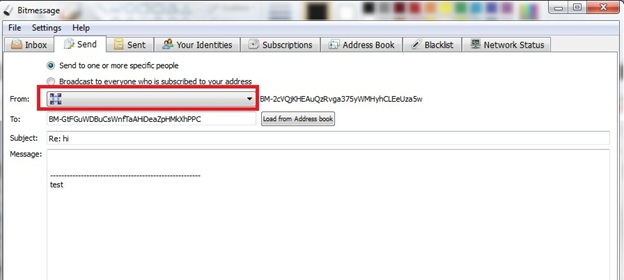
\includegraphics[width=12cm,height=5cm]{F2_4.jpg}}   
  \centering  \caption{Screen showing the 'from' field populated with corresponding icon}
  \end{center}
\end{figure}

%% Puskar


\section{Feature: Windows Installer}
\subsection {Introduction:}
% And that's what we call understanding.
\begin{enumerate}

\item Window Installer: 
Window installer is an installation and configuration service based on data driven model giving installation data and instruction in a single package which focuses on what to install. It is used in Microsoft windows system for software installation, software maintenance and software removal. The advantage of window installer is that they synchronize with other installers and consistency in installed product internal database. This feature allows user to install BitMessage in Windows system, provide optional shortcuts in common location, allow installer to ask if it should be started at login or not and auto-update new Bitmessage if new version of Bitmessage exists in authenticated server. BitMessage has two dependencies, PyQt and OpenSSL. Window installer include both dependencies so that user can install it in windows which doesnot have PyQt and OpenSSL and it allows user to install BitMessage in common locations, flexibility of starting application at login and auto-check for new version of Bitmessage and update it if new version exists. Simple and powerful language for scripting which supports various GUI packages makes python suitable to develop application. But during compilation of python project from idle, it doesnt create executable as in C\# , C++ etc. So, to create standalone executable from python project, separate plugin is required. Since PyQt and OpenSSL are two dependencies in BitMessage, proper handling of it during creation of executable should be done. PyInstaller is used to create executable from bitmessage project since it also support loading external dynamic link library so that we can resolve external dependencies.
To resolve OpenSSL DLL in exe, libeay32.dll is included in standalone executable. For the window installer, a script is written in pascal programming language which also includes standalone executable and compiled with open source setup compiler INNO setup. Moreover, auto-update feature of Bitmessage is written in C\#. 
\\
\item PyInstaller: 
PyInstaller is mutltiplatform program used to convert python program into executable which works with any version of python since 2.4. It also supports loading dynamic link library ensuring full compatibility. Main goal of pyinstaller is to integrate third party package along with executable ensuring all dependencies are satisfied.\\
\item INNO Setup:
 It is a free script-driven installation system for window programs. In terms of feature and stability, it is competitive and even surpasses some commercial software. The main advantage is that it support multilingual, Unicode and digitally signed installs and uninstalls. Other advantages are it supports every window after 2000 and extensive support for 64 bit windows as well. It also allows customizable setup like full, minimal or custom and helps to create uninstall capabilities.\\
 \item Auto-update: 
During installation, the version of the Bitmessage in text file is also downloaded. 
The auto-update feature checks the version of Bitmessage of local repository with the version of Bitmessage in authenticated server and update Bitmessage from authenticated remote server if new version exists over there. Authenticated web url’s are provided by Bitmessage contributor for auto-update feature. The window installer with auto-update feature is tested in the 32-bit and 64-bit window machine which doesn’t have python, PyQt and OpenSSL.
\begin{enumerate}
 \item \href{https://bitmessage.org/forum/index.php?topic=3316.msg6986#msg6986.html}{Forum Thread} 
 \item \href{https://github.com/Bitmessage/PyBitmessage/pull/585}{Pull Request} \end{enumerate}

\subsection{User Story}

Title: Window Installer\\
Description:As a window installer, it needs to be installed and configured in 32bit/64bit windows with
installation data and instruction in single package.
Similarly it should prompt the message to allow for optional shortcuts in common locations.\\
Acceptance criteria:
The installer package should include all dependencies like PyQt and OpenSSL and it should be compatible with both 32 bit and 64 bit windows. Similarly the user should complete all the procedure prompted in installation dialog box to complete the setup procedure.\\

Title: Auto-update of window installer \\
Description:The application should be able to auto-update in each startup to a newer version if new version exists.\\
Acceptance criteria:
The installer should be updated to newer version if the Bitmessage in local machine is of different version than the authenticated server Bitmessage.\\

\subsection{Changelog}
The setup scripting is written in pascal programming language and can be compiled with open source setup compiler INNO setup .Similarly auto-update feature is written in C\#. Change the location of "OutputDir" to user desired location to generate installer file and give location of BitUpdate.exe in "[Files] Source": in scripting file setup.iss. Compile it and get the Installer



\subsection{Step-wise guide to installation}
After we get the window installer from above process, the following steps should be done to complete installation
\begin{enumerate}

\item Window dialog box giving detail about installer information along with version is appeared.\\
\begin{figure}[H]
\begin{center}
    {\label{fig:1} 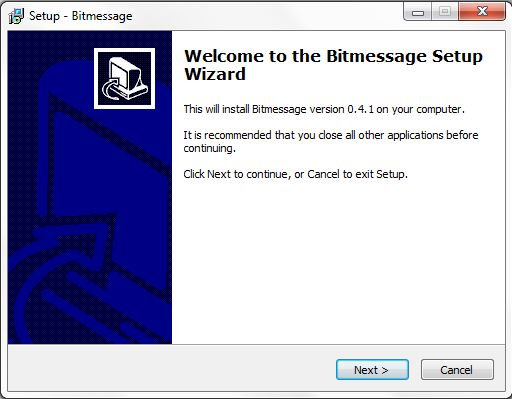
\includegraphics[width=7cm, keepaspectratio]{SE.jpg}}   
  \centering  \caption{Bitmessge window installer with version}
  \end{center}
\end{figure}

\item Window installer provides flexibility to install the application in any drive.\\
\begin{figure}[H]
\begin{center}
    {\label{fig:1} 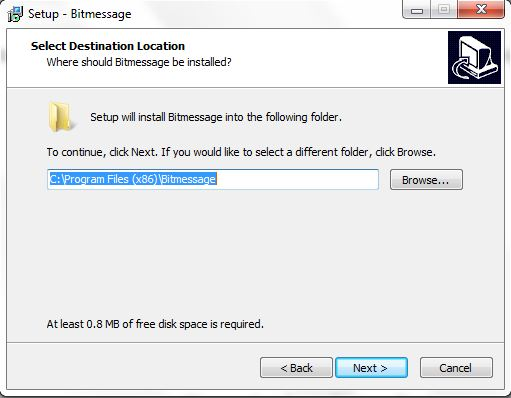
\includegraphics[width=7cm, keepaspectratio]{SE1.jpg}}   
  \centering  \caption{ Installation Path}
  \end{center}
\end{figure}

\item If the window installer is already installed in the path specified, it gives the information to user. 
\begin{figure}[H]
\begin{center}
    {\label{fig:1} 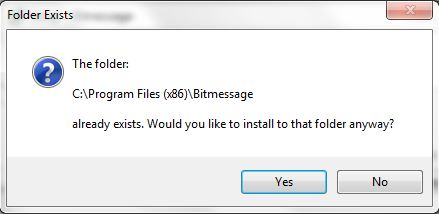
\includegraphics[width=7cm, keepaspectratio]{SE2.jpg}}   
  \centering  \caption{ Warning prompt}
  \end{center}
\end{figure}

\item It also provides flexibility to change the start menu name and the path. 
\begin{figure}[H]
\begin{center}
    {\label{fig:1} 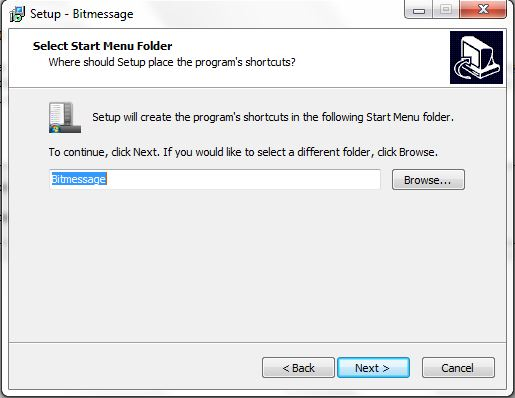
\includegraphics[width=7cm, keepaspectratio]{SE3.jpg}}   
  \centering  \caption{Start menu with installation path}
  \end{center}
\end{figure}



\item Installer allow for optional shortcuts in common locations like creating desktop icon.
\begin{figure}[H]
\begin{center}
    {\label{fig:1} 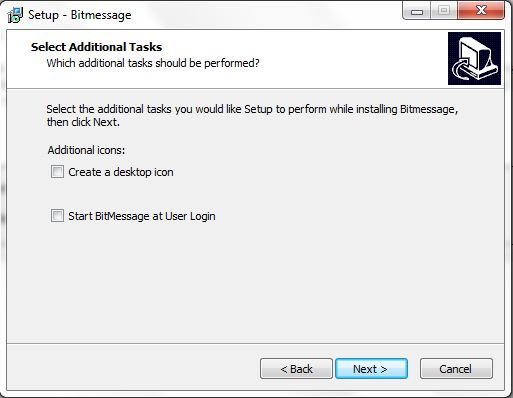
\includegraphics[width=7cm, keepaspectratio]{SE4.jpg}}   
  \centering  \caption{optional shortcut}
  \end{center}
\end{figure}

\item  Then after it  gives the summary of the whole installation process.\\ 
\begin{figure}[H]
\begin{center}
    {\label{fig:1} 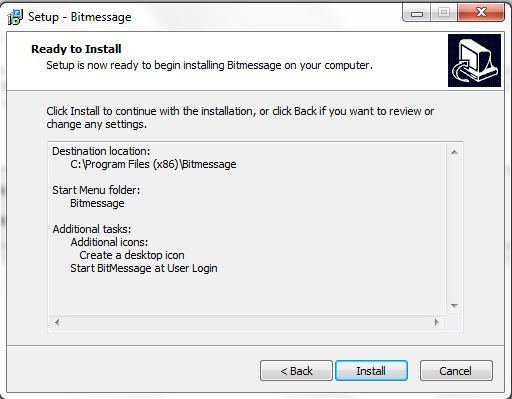
\includegraphics[width=7cm, keepaspectratio]{SE5.jpg}}   
  \centering  \caption{Installation summary}
  \end{center}
\end{figure}
\item  Finally it check version of Bitmessage from authenticated server and install window installer from it.\\ 
\begin{figure}[H]
\begin{center}
    {\label{fig:1} 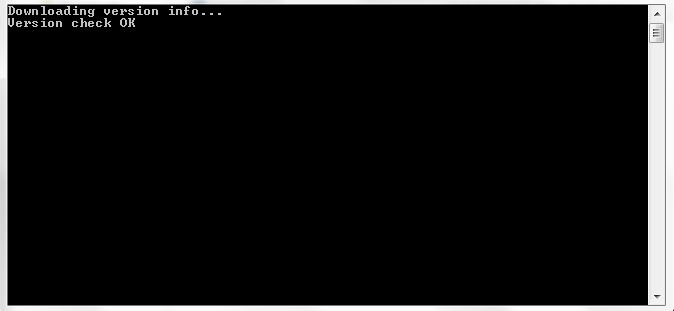
\includegraphics[width=7cm, keepaspectratio]{SE6.jpg}}   
  \centering  \caption{Installation progress}
  \end{center}
\end{figure}







\end{enumerate}
\end{enumerate}


\end{document}
